\documentclass{article}
\usepackage[english,american]{babel}
\usepackage{todonotes}
\usepackage{subfiles}
\usepackage{grffile}
\usepackage{booktabs}
\usepackage{hyperref}
\usepackage{fullpage}

\usepackage{csquotes}% Recommended
\usepackage{amssymb}
\usepackage{biblatex}

\usepackage{amsmath}
\usepackage{subcaption}
\usepackage{multicol}

\DeclareGraphicsRule{.ai}{pdf}{.ai}{}


\title{Spatial Relational Models for Neural Circuit Discovery}
\author{Eric Jonas \\ Konrad Kording}

\begin{document}
\maketitle

\listoftodos

\begin{abstract}
  The role of ``type''
  Clustering in molecular biology
\end{abstract}

\section{Introduction}

Things I believe

\begin{itemize}
\item The rise of complex data demands better computational tools to ``see'' into it
\item Clustering has worked for molecular biology and genetics
\item ``Type'' is a useful concept for understanding how neurobiological systems work
\item Many things people do with graphs are boring, not biologically relevant
\item Neuroanatomy needs to be a computational field
\end{itemize}

\section{Methods}
Stochastic blockmodels have been around forever, assume a latent ``type'' dictates
the probability of a latent class. We use recently-developed infinite
stochastic block models that 

\begin{figure}
  \centering 
  \begin{subfigure}[b]{0.4\textwidth}
    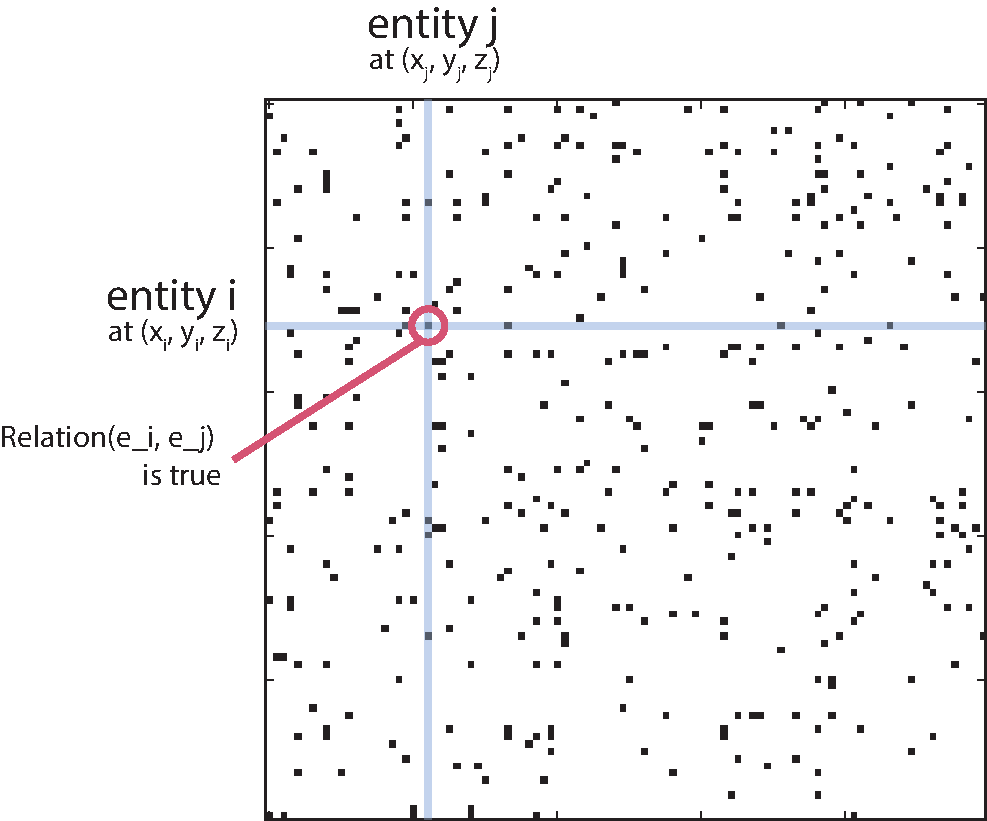
\includegraphics[width=\textwidth]{f1.raw.pdf}
    \caption{Raw data}
    \label{fig:gull}
  \end{subfigure}
  \begin{subfigure}[b]{0.55\textwidth}
    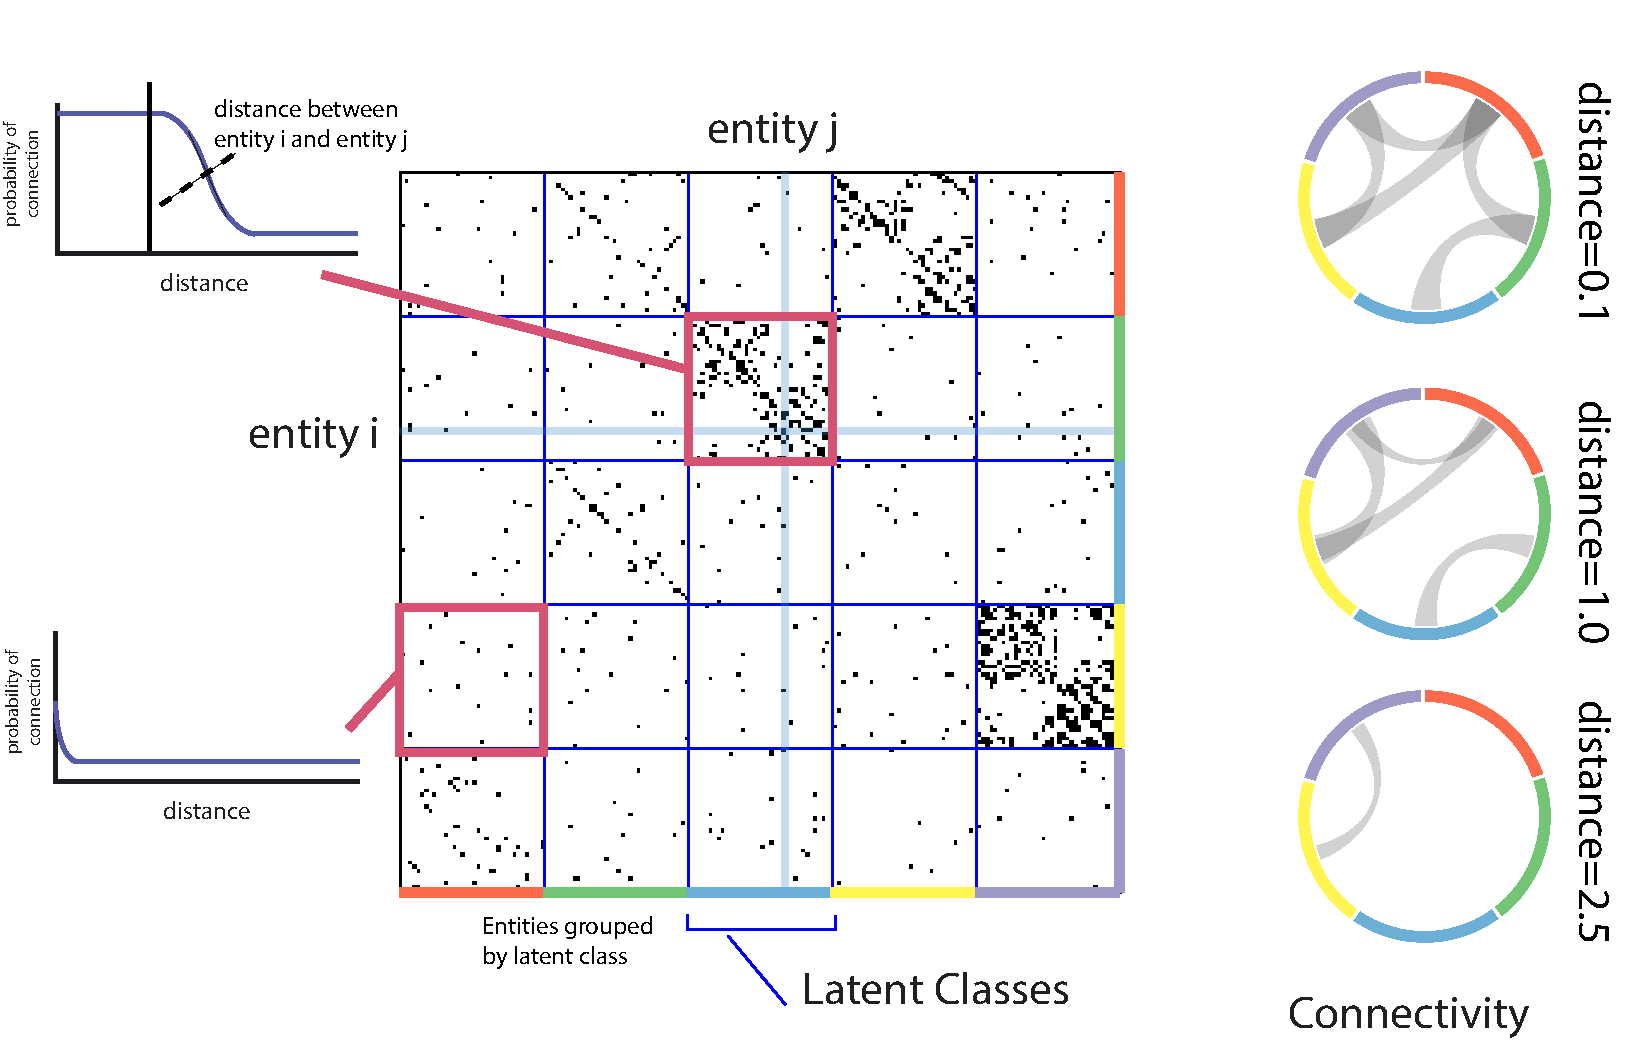
\includegraphics[width=\textwidth]{f1.sorted.pdf}
    \caption{Raw data}
    \label{fig:gull}
  \end{subfigure}
\end{figure}

\subsection{infinite Spatial Relational Models}

We adopt the terminology from \autocite{Kemp}. A domain $T_n$ is a
collection of entities $\{e^t_i | i \in 0 \dots N^t -1 \} $ that share
some common property. A relation is a collection of observation
defined on a collection of domains. For example, if one domain is
``students'' and another is ``courses'', the relation
``$\operatorname{has-taken}(e^s_i, e^c_j)$ is true if student $e^s_i$ has
taken course $e^c_j$. 

Our model assumes that the probabiltiy of a relation taking on a
particular observed value is only a function of some hidden ``type''
(or class, or cluster) of an entity. Each entity can belong to a
single latent class.

That is, if $e^1_i$ is an entity
in domain $T^1$ and in latent class $m$ and $e^2_j$ is an entity in
domain $T^2$ in latent class $n$, then 
\begin{equation}
\operatorname{Relation}(e^1_i, e^2_j) \sim F(\cdot | \eta_{mn})
\end{equation}

where $\eta_{mn}$ is an unobserved (latent) parameter.
\todo{Better framing of this}

Note that this framework is equivalent to the classic stochastic block
model, defined on a graph -- a relation $\operatorname{has-edge}(e_i,
e_j)$ is defined on the domain $T1$ of nodes. 

\subsubsection{Arbitrary discriminative funtions}
We can extend models of this type 

\begin{equation}
P(e_i, e_j) \sim F(g_{mn}(e_i, e_j))
\end{equation}

where $g_{mn}$ is an arbitrary link function $g$ defined per-latent
class -- if $e_i$ is of latent class $m$ and $e_J$ is of latent class
$n$, then the likelihood function $F$ is evaluated at $g_{mn}(e_i,
e_j)$ instead of a fixed parameter $\eta_{mn}$ in the classical
model. This allows an arbitrary discriminative function between
additional parameters of entities $e_i$ and $e_j$. That is, $g$ can be
defined on additional per-entity attributes, like spatial location.

We're principally interested in spatial models, so we associate with each
entity $e_i$ a location in space, and parameterize a per-latent-class
link function 
\todo{later}

\subsubsection{Infinite prior}
exchangability 
chinese restaurant process prior



\subsection{Likelihoods}
We evaluated a collection of link functions. 
Many of these are needed to map from $\mathbb{R}^+$ to some closed interval. 
TODO where do we talk about how this is like GLMs? 

Let $x_i$ and $x_j$ be the spatial locations of entities $e_i$ and $e_j$. $D(e_i, e_j$ is the euclidian distance between these two points. 
 
\subsubsection{Logistic Distance}
We use a binary observation for the relation (Bernoulli), and the $p$ is determined
on a per-class basis

prior on mu, lambda

\begin{figure}
  \centering 
  \begin{subfigure}[b]{0.4\textwidth}
    \includegraphics[width=0.3\textwidth]{logisticdistance.ai}
    \caption{Raw data}
    \label{fig:gull}
  \end{subfigure}

  \begin{subfigure}[b]{0.4\textwidth}
    \includegraphics[width=0.3\textwidth]{exponentialdistancepoisson.ai}
    \caption{Raw data}
    \label{fig:gull}
  \end{subfigure}

\end{figure}

This likeilihood model uses a logistic transform from distance to the
probability $p$ of a connection between two entities $e_i$ and
$e_j$. The latent class component parameters are the center of the
logistic $\mu_{mn}$ and the scale $\lambda_{mn}$. If the distance
between $e_i$ and $e_j$ is less than $\mu_{mn}$ then they are more
likely to be connected. To smooth out the likelihood, we scale the logistic
function by $p_{\textrm{min}}$ and $p_{\textrm{max}}$

So the generative model is
\[\mu_{ab} \sim \exp(\mu^{hp}) \]
\[\lambda{ab} \sim \exp(\lambda^{hp}) \]
\[p^* = \frac{1.0}{1.0 + \exp{\frac{(d(e_i, e_j) - \mu_{ab})}{\lambda_{mn}}}}\]
and then 
\[ r \sim \operatorname{Bernoulli}(p\cdot (p_{max} - p_{min}) + p_{min}) \]

\todo{example figure of parameterization, and notes}
We don't do hyperparameter inference on $p_{min}$ and $p_{max}$. 

\subsubsection{Normal Distance Fixed witdh}

\subsubsection{Exponential Distance Bernoulli}
\todo{Implement and test this model}


\subsubsection{Exponential Distance Poisson}
Some of our observations are count-valued. 


\subsubsection{Exponential Distance Normal}


\subsubsection{Non-spatial, Conjugate likelihoods for comparison}
Beta Bernoulli
Gamma-Poisson

\subsection{Inference}

We use Markov-chain Monte Carlo techniques to sample from the posterior 
distribution of our model conditioned on the data. Inference is
performed over cluster assignments, the per-component latent parameters, 
and the per-relation, datatype-specific parameters. 


\subsubsection{Structural Inference}
Algorithm 8 from radford neal \cite{nealalgo8}

\subsubsection{Per-component parameters in nonconjugate case}
Slice sample on latent parameters


\subsubsection{Hyperparameter Inferece}
Gridded gibbs sampling for hyperparameter inference

\subsubsection{Annealing}
For many examples of the data here we perform annealing. 



\section{Results}

\subsection{Synthetic Data}
Show that traditional stochastic block model fails. 


The goal of the synthetic results is to show that we recover ground truth. 
1. where is the data from? 
2. how did we generate it? 


\subsection{Mouse Retina}

Dense serial electron microscopy of a $VOLUMNE$ in the mouse
retina by \autocite{MouseReinta} yielded a listing of places where
neurons come into contact. There were $number$ cells originally, whcih
were refined through various classification schemes. We selected the
$NUMBER$ for which the location of the soma could be reconstruted from
the provided cell plots (soma locations were not provided by the
study's authors in machien-readble form).

The authors were unable to disambiguate actual ``synapses'' in the
full data set, but were able to measure the points of contact between
cells. Thus we don't have ``real'' synapses. We also don't have directionality. 


\subsection{C. elegans}
Connectome across several animals traced out by sidney brenner back in the day.
Small number of cells
position is linear along body axis
cell divisions are really precise

only look at hermaphrdite, ignore phyranx. 

Have directionality, chemical vs electrical, number


\subsection{Drosophila medulla}
\cite{DrosophilaConnectome}
No cell bodies -- what to use for distance? 
Human annotation
what the hell is a cell

\subsection{MOS 6502}

Hobbiest groups seeking to preserve historical microprocessors have
measured the ``connectomes'' of silicon integrated circuits. This
process involves obtaining classic chips, removing the casing
chemically, and then taking multi-gigapixel visible-light micrographs
of the silicon layers contained within. Then, a partially automated
process is used to read out the silicon polygons and reconstruct the
processor circuit contained within. The results are quite impressive,
with groups having successfully measured the original MOS6502 (Found
in the Apple I), and then used this ``connectome'' to perform
cycle-accruate simulation.

We extracted this data at the per-transistor level from the online
github project, resulting in $NUMBER$ transistors. Each transistor has
three terminals: $g$, $c_1$, and $c2$. Electronic circuits are fundamentally
undirected at the physical leve. 

Remove CLK, VCC/VSS. 

This would work better up one level of abstraction. 


Challenges: not directed. Three terminals. Dense connections. 

THIS SHOULD WORK

\subsection{Zipcode data}

This data is from career builder. It contains who applied to what jobs. This is our first non-graph example of a T1xT2 relation. 



\section{Discussion}
Do we have enough data to make this work? 

Why does it fail sometimes? 

Tendency of stochastic block models to have block-diagonal structure -- that's not really how neuro works

Is type a static thing or a continuum? 


\section{Next Steps / Future Work}
How in gods name do we evaluate this? 

What abotu mixed membership models / better structural priors

What about incorporating additional metadata (``attribtue'' data)

Can we use something like a GP to learn the link function? 
Parametric link functions are nice, but you'd like to learn it from the data

How in gods name do we make this scale to 100k nodes? 
VB? spectral methods? Shitty heuristics? 

How in gods name do we make this hierarchical? 
We expect there to be hierarchy 

\end{document}




